\documentclass[letterpaper, 10 pt, conference]{ieeeconf}
\IEEEoverridecommandlockouts % This command is only needed if
% you want to use the \thanks command

\overrideIEEEmargins % Needed to meet printer requirements.

% See the \addtolength command later in the file to balance the column
% lengths on the last page of the document
\usepackage{microtype}
% The following packages can be found on http:\\www.ctan.org
% \usepackage{graphics} % for pdf, bitmapped graphics files
% \usepackage{epsfig} % for postscript graphics files
% \usepackage{mathptmx} % assumes new font selection scheme installed
% \usepackage{times} % assumes new font selection scheme installed
% \usepackage{amsmath} % assumes amsmath package installed
% \usepackage{amssymb} % assumes amsmath package installed

\usepackage[pdftex,pdfauthor={MFE},pdftitle={6.867 Final Project}]{hyperref}
\hypersetup{colorlinks,linkcolor={green!50!black},citecolor={green!50!black},urlcolor={blue!80!black}}
\makeatletter \let\NAT@parse\undefined \makeatother
% \usepackage[square,comma,sort&compress]{natbib}
\usepackage[sort,compress]{cite}
\usepackage{graphicx} % more modern
\usepackage{amsfonts}
\usepackage{amsmath,soul}
\usepackage{color}
\usepackage[font=small]{subcaption}
\usepackage{balance}
\usepackage[font=small]{caption}
%\usepackage{subfigure,balance}
%\usepackage[colorlinks=true]{hyperref}
%\usepackage{subcaption,balance}
\usepackage[noend]{algorithmic}
\usepackage[linesnumbered,ruled,vlined]{algorithm2e}
\usepackage{multirow}

% from bjorn:
\usepackage{xfrac}
\usepackage{mathtools}
\usepackage{bm}


\DeclareMathOperator*{\argmin}{\arg\!\min}
\DeclareMathOperator*{\argmax}{\arg\!\max}
\usepackage{tabulary}
\newcolumntype{K}[1]{>{\centering\arraybackslash}p{#1}}


\newtheorem{definition}{Definition}
\newtheorem{assumption}{Assumption} \newtheorem{theorem}{Theorem}
\newtheorem{lemma}{Lemma}
\newtheorem{corollary}[theorem]{Corollary}

\title{\LARGE \bf Pedestrian Motion Classification for Autonomous Vehicles\\(6.867 Final Project)}

\author{Michael Everett \& Bj{\"o}rn L{\"u}tjens}

% \usepackage[usenames]{color}
%\DeclareMathOperator*{\argmin}{arg\,\!min}
%\DeclareMathOperator*{\argmax}{arg\,\!max}
\usepackage[svgnames]{xcolor} \definecolor{DarkGreen}{rgb}{0,0.5,0}
\definecolor{DarkRed}{rgb}{0.75,0,0}

\usepackage[authormarkuptext=name,addedmarkup=bf,authormarkupposition=left]{changes}
%\usepackage[final]{changes} %Use this to hide all comments.
\definechangesauthor[name={M.~E.}, color={red}]{me}
\setremarkmarkup{(#2)}

\newcommand{\XX}[1]{\added[id=jh,remark={}]{#1}}
\newcommand{\jmXX}[1]{\added[id=jm,remark={}]{#1}}
\newcommand{\meXX}[1]{\added[id=me,remark={}]{#1}}

\newcommand{\jsec}[1]{\marginpar{\fcolorbox{yellow}{yellow}{\parbox{0.7in}{\raggedright
        \color{blue} \tiny #1 }}}}
\newcommand{\hsec}[1]{\marginpar{\fcolorbox{yellow}{yellow}{\parbox{0.7in}{\raggedright
        \color{green} \tiny #1 }}}}
\newcommand{\jhmargin}[2]{{\color{orange}#1}\marginpar{\color{orange}\tiny\raggedright
    \bf [JH] #2}}


\usepackage{tikz,mathtools}
%\usepackage{cleveref}
\usepackage[capitalize]{cleveref}
\crefformat{equation}{(#2#1#3)}
\Crefformat{equation}{Equation~(#2#1#3)}
\Crefname{equation}{Equation}{Equations}

\newcommand{\inputTikZ}[2]{\scalebox{#1}{\input{#2}}}
\usetikzlibrary{shapes,positioning,automata,arrows,fit,backgrounds,calc}
\tikzstyle{block} = [draw, fill=blue!20, rectangle,minimum height=1em,
minimum width=2em] \tikzstyle{sum} = [draw, fill=blue!20, circle, node
distance=1cm] \tikzstyle{input} = [coordinate] \tikzstyle{output} =
[coordinate] \tikzstyle{pinstyle} = [pin edge={to-,thin,black}]
\usetikzlibrary{trees} \usetikzlibrary{decorations.pathmorphing}
\usetikzlibrary{decorations.markings}
\definecolor{darkgreen}{rgb}{0,0.5,0}
\definecolor{darkred}{rgb}{220,20,60}

\makeatletter
\renewcommand\paragraph{\@startsection{subsubsection}{4}{\z@}%
{0.25ex \@plus.5ex \@minus.2ex}%
{-.15em}%
{\normalfont\normalsize\itshape}}
\makeatother


\begin{document}

\maketitle
\thispagestyle{empty} \pagestyle{empty}

% %%%%%%%%%%%%%%%%%%%%%%%%%%%%%%%%%%%%%%%%%%%%%%%%%%%%%%%%%%%%%%%%%%%%%%%%%%%%%%%

\begin{abstract}
In this project, we applied techniques from the course to a dataset of pedestrian trajectories recorded on a golf cart around MIT's campus.
Our objective was to classify whether a pedestrian's trajectory would enter a 4x10m rectangle in front of the vehicle, which could be used as an active safety feature on various types of vehicles that interact with pedestrians.
We trained a SVM with Gaussian RBF Kernel and optimized hyperparameters to achieve 86.3\% test accuracy.
We then trained an RNN for the same task and achieved \meXX{RNN accuracy?} accuracy.
Finally, we experimented with pedestrian motion prediction, to predict the future pedestrian trajectory.
\end{abstract}

%%%%%%%%%%%%%%%%%%%%%%%%%%%%%%%%%%%%%%%%%%%%%%%%%%%%%%%%%%%%%%%%%%%%%%%%%%%%%%%%
\section{Introduction} \label{sec:intro}

% \XX{do you cite olson??} \sXX{now cited}

% applications of socially aware navigation (robots)
Recent advances in sensing and computing technologies have spurred greater interest in various applications of autonomous ground vehicles. In particular, researchers have explored using robots to provide personal mobility services and luggage carrying support in complex, pedestrian-rich environments (e.g., airports and shopping malls)~\cite{bai_intention-aware_2015}. These tasks often require the robots to be capable of navigating efficiently and safely in close proximity of people, which is challenging because pedestrians tend to follow subtle social norms that are difficult to quantify, and pedestrians' intents (i.e., goals) are usually not known~\cite{kretzschmar_socially_2016}.

% prediction + static motion planner -> freezing robot problem
A common approach treats pedestrians as dynamic obstacles with simple kinematics, and employs specific reactive rules for avoiding collision~\cite{fox_dynamic_1997,van_den_berg_reciprocal_2008,phillips_sipp:_2011,berg_reciprocal_2011}. Since these methods do not capture human behaviors, they sometimes generate unsafe/unnatural movements, particularly when the robot operates near human walking speed~\cite{kretzschmar_socially_2016}. To address this issue, more sophisticated motion models have been proposed, which would reason about the nearby pedestrians' hidden intents to generate a set of predicted paths~\cite{kim_brvo:_2015,unhelkar_human-robot_2015}. Subsequently, classical path planning algorithms would be employed to generate a collision-free path for the robot. Yet, separating the navigation problem into disjoint prediction and planning steps can lead to the \emph{freezing robot problem}, in which the robot fails to find any feasible action because the predicted paths could mark a large portion of the space untraversable~\cite{trautman_robot_2015}.
%\mXX{they have a newer journal paper extending the freezing robot problem, which might worth citing, \url{http://journals.sagepub.com/doi/pdf/10.1177/0278364914557874.}} \sXX{added reference to this new work}
A key to resolving this problem is to account for cooperation, that is, to model/anticipate the impact of the robot's motion on the nearby pedestrians. 

\begin{figure}[t]
	\centering
%	\includegraphics [trim=0 0 0 0, clip, angle=0, width=0.8\columnwidth, keepaspectratio]{figures/stata_nav}
	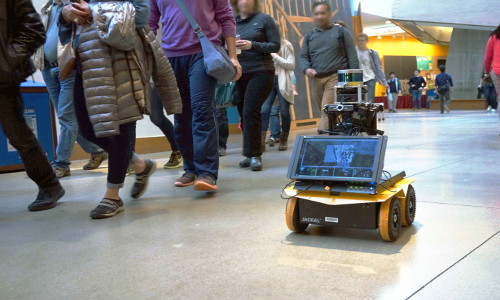
\includegraphics [trim=0 0 0 0, clip, angle=0, width=0.8\columnwidth,
	keepaspectratio]{figures/rover_d}
	\caption{A robotic vehicle navigating autonomously in a pedestrian-rich environment. Accounting for social interactions is important for operating such vehicles safely and smoothly. %\sXX{will take a better pic}
	} 
	\label{fig:rover} 
	%\vskip -0.1in
\end{figure}

%\XX{\color{red} many weak sentences in the following - make it sharper and more clear} \sXX{reworded}
% cooperative methods (behabivor approach - BRVO, social forces)
%Existing work on cooperative, socially compliant navigation can be broadly classified into two categories, namely \textit{model-based} and \textit{learning-based}. Model-based approaches are typically extensions of multiagent collision avoidance algorithms, with additional tuned parameters to account for human--human and human--robot interactions~\cite{helbing_social_1995,ferrer_robot_2013,kim_brvo:_2015}. These methods \XX{are computationally efficient, - how do you know? seems like an odd statement - it might be how they re designed} but \XX{might not capture - \color{red} not a great statement at all} the complexity of human behaviors. In particular, \XX{the parameters - we don't know what you are talking about here} can vary 
%\XX{do you mean that the parameter settings needed can be highly dependent on the scenario and the particular pedestrians??}
%significantly among pedestrians and these methods can lead to generating oscillatory trajectories~\cite{kretzschmar_socially_2016,chen_decentralized_2017}.

Existing work on cooperative, socially compliant navigation can be broadly classified into two categories, namely \textit{model-based} and \textit{learning-based}. Model-based approaches are typically extensions of multiagent collision avoidance algorithms, with additional parameters introduced to account for social interactions~\cite{helbing_social_1995,ferrer_robot_2013,ferrer_behavior_2014,kim_brvo:_2015,mehta_autonomous_2016}. For instance, to distinguish between human--human and human--robot interactions, the extended social forces model~\cite{ferrer_behavior_2014,ferrer_robot_2013} augments the potential field algorithm with additional terms that specify the repulsive forces (e.g., strength and range) governing each type of interaction. Model-based methods are designed to be computationally efficient as they often correspond to intuitive geometric relations; yet, it is unclear whether humans do follow such precise geometric rules. In particular, the force parameters often need to be tuned individually, and can vary significantly for different pedestrians~\cite{ferrer_behavior_2014}. Also, it has been observed that model-based methods can lead to oscillatory paths~\cite{chen_decentralized_2017,kretzschmar_socially_2016}. %Recent work has proposed switching between a few model-based approaches~\cite{mehta_autonomous_2016}, which can lead to having more parameters to tune. 

% cooperative methods (learning based approach - inverse RL, max entropy)
In comparison, learning-based approaches aim to develop a policy that emulates human behaviors by matching feature statistics, such as the minimum separation distance to pedestrians. In particular, Inverse Reinforcement Learning (IRL)~\cite{abbeel_apprenticeship_2004} has been applied to learn a cost function from human demonstration (teleoperation)~\cite{kim_socially_2015}, and a probability distribution over the set of joint trajectories with nearby pedestrians~\cite{kuderer_feature-based_2012,kretzschmar_socially_2016}. Compared with model-based approaches, learning-based methods have been shown to produce paths that more closely resemble human behaviors, but often at a much higher computational cost. This is because computing/matching trajectory features often requires anticipating the joint paths of all nearby pedestrians~\cite{kretzschmar_socially_2016}, and might depend on some  unobservable information (e.g., pedestrians' goals). 
%5
More importantly, since human behaviors are inherently stochastic, 
%\XX{paths - is the issue here paths or behaviors? my path might change even though my behavior doesn't} \sXX{the feature statistics can differ due to stochasticity in people's behavior, so feature matching won't work/generalize so well. } 
the feature statistics calculated on pedestrians' paths can vary significantly from person to person, and even run to run for the same scenario~\cite{kim_socially_2015,kretzschmar_socially_2016}. This raises concerns over whether such feature-matching methods are generalizable to different environments~\cite{mehta_autonomous_2016}.

% main challenge
%\mXX{The transition seems not smooth. previous two paragraphs talked two categoies of methods and their issues. Might want to remind reader that the proposed method is also learning based or something else and those issues in the previous methods} \sXX{good point, need to address this comment}
%In short, due to the stochasticity in people's behaviors, socially compliant navigation remains difficult to quantify despite being instinctive to humans. \XX{thought flow from last sentence to here doesn't make sense} Yet, it has been widely observed that human navigation (or teleoperation) is time-efficient and generally respects a set of simple social norms (i.e., ``passing on the right'')~\cite{kim_socially_2015,kretzschmar_socially_2016,knepper_pedestrian-inspired_2012}. We note that while it is challenging to directly specify the details of \emph{what to do} (precise mechanisms of human navigation), it is straightforward to specify \emph{what not to do} (violations of social norms).

In short, existing works are mostly focused on modeling and replicating the detailed mechanisms of social compliance, which remains difficult to quantify due to the stochasticity in people's behaviors. In comparison, humans can intuitively evaluate whether a behavior is acceptable. In particular, human navigation (or teleoperation) is time-efficient and generally respects a set of simple social norms (e.g., ``passing on the right'')~\cite{kim_socially_2015,kretzschmar_socially_2016,knepper_pedestrian-inspired_2012}. %Moreover, we note that while it is challenging to directly specify the details of \emph{what to do} (precise mechanisms of human navigation), it is straightforward to specify \emph{what not to do} (violations of social norms). 
Building on a recent paper~\cite{chen_decentralized_2017}, we characterize these properties in a reinforcement learning framework, and show that human-like navigation conventions emerge from solving a cooperative collision avoidance problem.
%\mXX{There are a few another popular Deep RLs, which we should use for comparison. Maybe for future journal submissions} \sXX{will investigate in future}

% CADRL, contributions
The main contributions of this work are 
%\XX{this is something you did - does not read as a contribution} \sXX{reworded}
(i) introducing socially aware collision avoidance with deep reinforcement learning (SA-CADRL) for explaining/inducing socially aware behaviors in a RL framework, (ii) generalizing to multiagent ($n>2$) scenarios through developing a symmetrical neural network structure, and (iii) demonstrating on robotic hardware autonomous navigation at human walking speed in a pedestrian-rich environment. 












%!TEX root = main.tex

\section{Dataset} \label{sec:dataset}

% where did dataset come from (cite justin's papers)

% what does raw data look like?
The raw dataset's fields are shown in \cref{table_data}, where (easting,northing) are the latitude/longitude global coordinates, and (x,y) are the coordinates in our global campus map.
Veh id indicates which of the three vehicles corresponds to that data point, or in the pedestrian case, which vehicle sensed that pedestrian, and ped id is a unique id given to each pedestrian seen.

\begin{table}[ht!]
\centering
\begin{tabular}{||c||c c c c c c c||}  
 \hline
 \multirow{1}{*}{Type} &
       \multicolumn{7}{c||}{Fields} \\
 \hline\hline
 Vechicle & time & easting & northing & x & y & veh id & \\ \hline
 Pedestrian & time & easting & northing & x & y & veh id & ped id \\ \hline
\end{tabular}
\caption{Raw data fields}
\label{table_data}
\end{table}

% what are the issues with the raw data
There are some noise-related issues with the raw data, as it was collected on a research vehicle under development.
One issue is that the vehicle's (x,y) position sometimes jumps, because the vehicle's localization system does not use GPS and is imperfect.

In addition to addressing noise, the data also needs to be pre-processed to be useful for our classifier.
Specifically, the pedestrian trajectories must be converted into the vehicle's local frame in order to determine if they cross in front of the vehicle.

% what is strategy to fix issues
The global-to-local transformation relies on knowledge of vehicle orientation (heading angle) and smooth vehicle trajectories, neither of which we have by default.

\begin{algorithm}
 \caption{Algorithm for ...}
 \begin{algorithmic}[1]
 \renewcommand{\algorithmicrequire}{\textbf{Input:}}
 \renewcommand{\algorithmicensure}{\textbf{Output:}}
 \REQUIRE global vehicle/pedestrain trajectories~(\cref{table_data})
 \ENSURE  pedestrian trajectories in local vehicle frame
 \\ \textit{Initialization} :
  \STATE first statement
 \\ \textit{LOOP Process}
  \FOR {$i = l-2$ to $0$}
  \STATE statements..
  \IF {($i \ne 0$)}
  \STATE statement..
  \ENDIF
  \ENDFOR
 \RETURN $P$ 

 \end{algorithmic} 
 \end{algorithm}

% what does fixed dataset look like



%!TEX root = main.tex

\section{SVM Binary Classifier} \label{sec:svm}

We trained a Support Vector Machine (SVM) to do binary classification on local pedestrian trajectories, to predict whether the trajectory will/will not enter a 4x10m rectangle in front of the vehicle.
A portion of the pedestrian trajectory is fed into the classifier, and it outputs a binary label.
This could be a useful safety feature on a car to identify which pedestrians might cross in front of the vehicle.

The trajectories are all of different length, so we split them up into equal ``snippets'' of length $l$.
Each trajectory has a single 0/1 label, and this same label is applied to each snippet.
This allows us to learn some notion of direction from (x,y) sequences, because a snippet that never crosses in front of the vehicle can still be labeled as such, if a later portion of its trajectory eventually does cross in front.
These $l$-long lists of (x,y) points are fed into the classifier as the feature vector of length $2l$, as:
$(x_i = [x_1, y_1, x_2, y_2, ... , x_l, y_l]; y_i = 0/1)$.

We used the SKLearn implementation of SVM~\cite{scikit-learn} with Gaussian RBF Kernel.

\subsection{Simple Example}
We first tried training with $l=1$, so that we could easily visualize the decision boundary in~\cref{fig:svm_snippet1}.
The data (magenta/cyan) aren't particularly meaningful, because it's hard to learn anything from a single (x,y) position of a pedestrian ($l=1$).
But, we can observe that the green decision boundary roughly resembles our arbitrarily-created rectangular ``cross zone''.
This figure indicates the SVM is correctly learning that there is a region in space that causes trajectories to be labeled a certain way.
After this quick sanity check, we can proceed to larger values of $l$, but lose the ability to easily visualize the results.

\begin{figure}
	\centering
	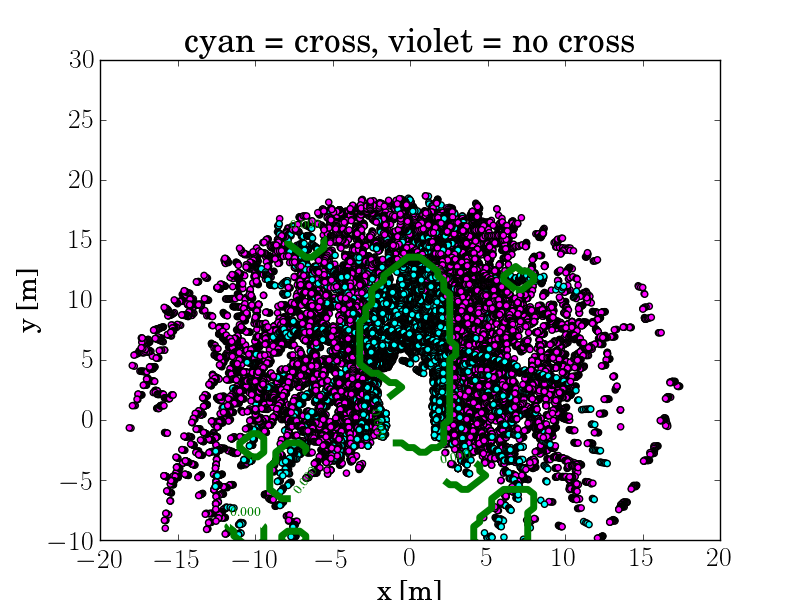
\includegraphics [trim=0 0 0 0, clip, angle=0, width=0.8\columnwidth,
	keepaspectratio]{figures/svm_snippet1}
	\caption{SVM trained on snippets with $l=1$ allow visualization of decision boundary. The important part of this plot is the green decision boundary in the center that resembles our arbitrary ``cross zone''. The SVM has roughly learned the location/shape of zone for simple input data. There is some overfitting evident by other green regions, but this is likely more of an artifact of $l=1$ hyperparameter.} 
	\label{fig:svm_snippet1} 
\end{figure}

\subsection{Hyperparameters}
There are several hyperparameters that affect the behavior of the classifier.
The main ones that we experimented with were $l$ (snippet length) and $C$ (SVM regularizer).
A grid search for optimal parameter values is shown in~\cref{table_svm} (optimal w.r.t. high validation accuracy).
Beacuse of the time required to train so many combinations (especially affected by Gaussian RBF Kernel), we trained on a smaller subset of the training set during hyperparameter optimization.

As $C$ increases, training accuracy increases for all scenarios, which is expected because this corresponds to more penalty on mis-classified points.
We can tell when $C$ is too high, because training accuracy is much higher than validation accuracy, a symptom of overfitting.

As $l$ increases, more time steps of pedestrian positions are used in the feature vector, so there is more information on which to classify.
Intuitively, large $l$ would seem preferable than small, but if $l$ is too large, the noise in the data may outweigh the value of the information.
To be more concrete, it seems unlikely that one would need 50 points worth of trajectory data to do the binary classification (especially given the noise seen in~\cref{fig:training_set}).

This intuition aligns with our observed validation accuracies.
The highest validation accuracy of 79.8\% occurs with $l=25$ and $C=10$, so we choose those as the optimal hyperparameters.

The test accuracy with these values was 74.4\%.

\begin{table*}[ht!]
\centering
\begin{tabular}{||c| c c c c c c c| c c c c c c c||}  
 \hline
 \multirow{2}{*}{Dataset} &
       \multicolumn{7}{c|}{$l=2$} &
       \multicolumn{7}{c||}{$l=10$} \\
 & $C=10^{-3}$ & $10^{-2}$ & $10^{-1}$ & $10^{0}$ & $10^{1}$ & $10^{2}$ & $10^{3}$ & $10^{-3}$ & $10^{-2}$ & $10^{-1}$ & $10^{0}$ & $10^{1}$ & $10^{2}$ & $10^{3}$ \\ [0.5ex] 
 \hline\hline
 Train & 70.8 & 83.2 & 84.8 & 85.9 & 87.1 & 89.1 & 91.9 & 63.8 & 76.1 & 84.6 & 86.8 & 92.6 & 97.2 & 99.6  \\ \hline
 Val & 63.1 & 77.4 & 79.1 & 78.9 & 78.0 & 77.8 & 77.6 & 60.3 & 67.9 & 78.4 & 79.4 & 79.3 & 77.7 & 76.1  \\ \hline
\end{tabular}
\begin{tabular}{||c| c c c c c c c| c c c c c c c||}  
 \hline
 \multirow{2}{*}{Dataset} &
       \multicolumn{7}{c|}{$l=25$} &
       \multicolumn{7}{c||}{$l=50$} \\
 & $C=10^{-3}$ & $10^{-2}$ & $10^{-1}$ & $10^{0}$ & $10^{1}$ & $10^{2}$ & $10^{3}$ & $10^{-3}$ & $10^{-2}$ & $10^{-1}$ & $10^{0}$ & $10^{1}$ & $10^{2}$ & $10^{3}$ \\ [0.5ex] 
 \hline\hline
 Train & 62.9 & 64.9 & 82.4 & 88.7 & 96.8 & 99.9 & 100 & 60.4 & 60.4 & 77.6 & 92.2 & 99.3 & 100 & 100  \\ \hline
 Val & 59.2 & 59.3 & 75.0 & 79.7 & 79.8 & 78.8 & 78.8 & 52.3 & 52.3 & 64.8 & 75.0 & 74.8 & 74.5 & 74.5  \\ \hline
\end{tabular}
\caption{Accuracy of SVM for various values of hyperparameters $C$, $l$.}
\label{table_svm}
\end{table*}

\subsection{Results}
With these optimized hyperparameters, we then trained on 1 week of data (9700 trajectory snippets).
The test accuracy was 84.8\%.
This is higher than the accuracy from hyperparameter optimization because there was more training data.

We show the various combinations of true/predicted labels in~\cref{fig:svm_labels}, with numerical listings in~\cref{table_svm_outputs}.
On the left (\cref{fig:svm_label0}), we show the trajectory snippets for which our classifier predicted a label of 0.
Our accuracy on trajectories that don't cross in front of the vehicle are pretty high.
It is interesting to note the rectangular gap in the center; this demonstrates that our classifier learned that trajectories that enter that region should never be classified as 1.
There are some red trajectories around the edge of the rectangle which are particularly challenging. 

On the right (\cref{fig:svm_label1}), the trajectories our classifier labeled as 1 are relatively somewhat less accurate.
Recall that the trajectories are split into snippets, so for long trajectories that are split into many snippets, this classifier seems to perform much worse on the snippets that are far away from the vehicle.
It is expected that the performance would be worse further away from the vehicle.
Some of the long trajectories are still classified correctly, indicating the classifier is learning some notion of direction, since we are only feeding in pedestrian positions over time.

\begin{table}[ht!]
\centering
\begin{tabular}{||c||c c||}  
 \hline
 Classification & Number & Percent \\
 \hline\hline
 False Positives & 101 & 4.6 \\ \hline
 False Negatives & 234 & 10.6 \\ \hline
 True Positives & 787 & 35.8 \\ \hline
 True Negatives & 1076 & 49.0 \\ \hline\hline
 Total & 2198 & 100.0\\ \hline
\end{tabular}
\caption{Classification matrix}
\label{table_svm_outputs}
\end{table}

\begin{figure}
\centering
\begin{subfigure}{.25\textwidth}
  \centering
  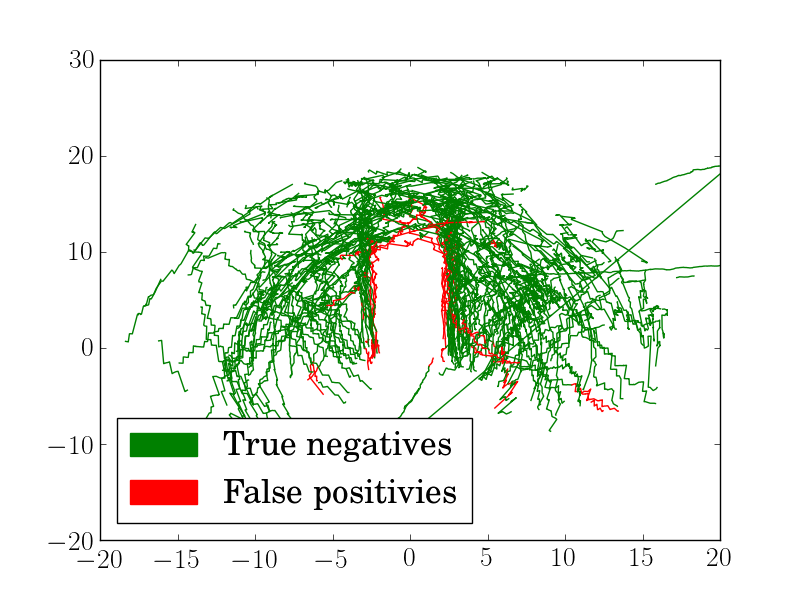
\includegraphics[width=.9\linewidth]{figures/svm_label0}
  \caption{Trajs. labeled ``No Cross''}
  \label{fig:svm_label0}
\end{subfigure}%
\begin{subfigure}{.25\textwidth}
  \centering
  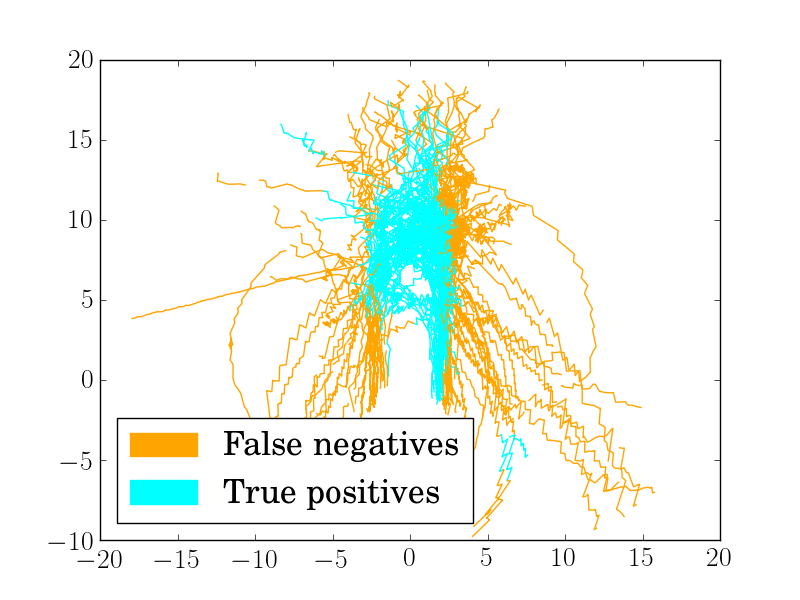
\includegraphics[width=.9\linewidth]{figures/svm_label1}
  \caption{Trajs. labeled ``Cross''}
  \label{fig:svm_label1}
\end{subfigure}
\caption{Predicted labels on test set with SVM classifier. On the left, trajectory snippets that were predicted label 0 (green is correct, red is incorrect). Notice the large rectangular gap in the center, corresponding to learned ``cross zone''. On the right, trajectory snippets that were predicted label 1 (cyan correct, orange incorrect). Across the whole test set, 84\% accuracy was achieved.}
\label{fig:svm_labels}
\end{figure}

\subsection{Kernel Choice}
According to~\cite{Rüping01svmkernels}, time series data can be classified with a SVM with many different types of kernels, but the most broadly applicable one is Gaussian RBF.
Therefore, we used a Gaussian RBF kernel with $\gamma$ set automatically by SKLearn's implementation.
This kernel allows non-linear combinations of feature elements, which could be useful for this task.
Ideally, we would use some kernel that was designed specifically for our time-series trajectory data, but we didn't focus much on this aspect of the problem.
Instead, we considered a different learning method (RNN) to try to better capture the time dependence of our data.


% t_steps: 2, C: 0.001000, Train: 0.708, Val: 0.631, Test: 0.590
% t_steps: 2, C: 0.010000, Train: 0.832, Val: 0.774, Test: 0.724
% t_steps: 2, C: 0.100000, Train: 0.848, Val: 0.791, Test: 0.733
% t_steps: 2, C: 1.000000, Train: 0.859, Val: 0.789, Test: 0.728
% t_steps: 2, C: 10.000000, Train: 0.871, Val: 0.780, Test: 0.721
% t_steps: 2, C: 100.000000, Train: 0.891, Val: 0.778, Test: 0.717
% t_steps: 2, C: 1000.000000, Train: 0.919, Val: 0.776, Test: 0.723

% t_steps: 10, C: 0.001000, Train: 0.638, Val: 0.603, Test: 0.555
% t_steps: 10, C: 0.010000, Train: 0.761, Val: 0.679, Test: 0.643
% t_steps: 10, C: 0.100000, Train: 0.846, Val: 0.784, Test: 0.732
% t_steps: 10, C: 1.000000, Train: 0.868, Val: 0.794, Test: 0.739
% t_steps: 10, C: 10.000000, Train: 0.926, Val: 0.793, Test: 0.736
% t_steps: 10, C: 100.000000, Train: 0.972, Val: 0.777, Test: 0.725
% t_steps: 10, C: 1000.000000, Train: 0.996, Val: 0.761, Test: 0.711

% t_steps: 25, C: 0.001000, Train: 0.629, Val: 0.592, Test: 0.542
% t_steps: 25, C: 0.010000, Train: 0.649, Val: 0.593, Test: 0.546
% t_steps: 25, C: 0.100000, Train: 0.824, Val: 0.750, Test: 0.709
% t_steps: 25, C: 1.000000, Train: 0.887, Val: 0.797, Test: 0.746
% t_steps: 25, C: 10.000000, Train: 0.968, Val: 0.798, Test: 0.744
% t_steps: 25, C: 100.000000, Train: 0.999, Val: 0.788, Test: 0.730
% t_steps: 25, C: 1000.000000, Train: 1.000, Val: 0.788, Test: 0.730

% t_steps: 50, C: 0.001000, Train: 0.604, Val: 0.569, Test: 0.523
% t_steps: 50, C: 0.010000, Train: 0.604, Val: 0.569, Test: 0.523
% t_steps: 50, C: 0.100000, Train: 0.776, Val: 0.676, Test: 0.648
% t_steps: 50, C: 1.000000, Train: 0.922, Val: 0.804, Test: 0.750
% t_steps: 50, C: 10.000000, Train: 0.993, Val: 0.818, Test: 0.748
% t_steps: 50, C: 100.000000, Train: 1.000, Val: 0.808, Test: 0.745
% t_steps: 50, C: 1000.000000, Train: 1.000, Val: 0.808, Test: 0.745

%!TEX root = main.tex
%TODO Figure 4: trajectories are not continuous because of snipping them. That's why a red traj is red and outside the collision area.

\section{Recurrent Neural Network: Binary classification} \label{sec:rnn_clf}

We first briefly describe RNNs and LSTMs, as these were not covered in homework assignments.
Then, we analyze the performance of an LSTM for the same binary classification task as before, and compare with the SVM implementation.

\subsection{Brief Overview of RNNs}

Recurrent Neural Networks (RNNs) have been shown to extract sequential information and generate highly complex sequences as documents, translations, music and more. 

\begin{figure}
	\centering
	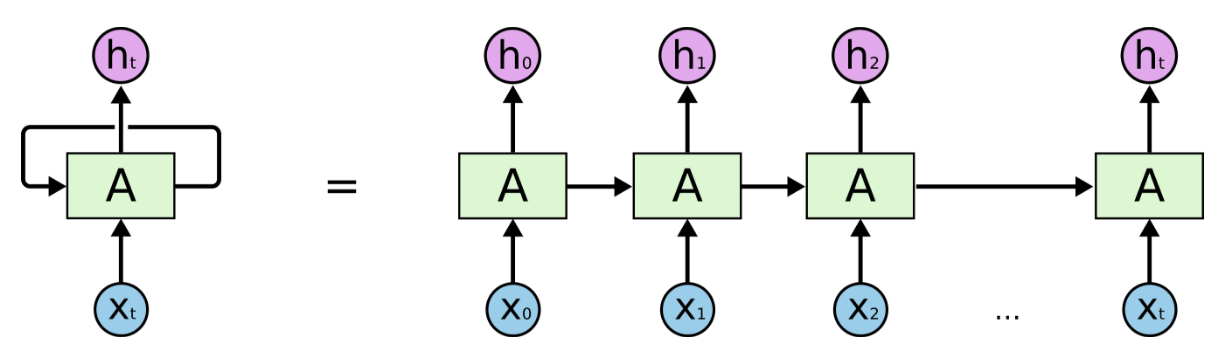
\includegraphics [trim=0 0 0 0, clip, angle=0, width=0.8\columnwidth,
	keepaspectratio]{figures/rnn_unrolled}
	\caption{Illustration of a RNN in it's enrolled (left) and unrolled (right) form. Each sequential input $x_t$ is fed in at timestep $t$, transformed by the activation cell $A$ and output and fed into the next cell as hidden state $h_t$. From~\cite{colah_lstm}} 
	\label{fig:rnn_unrolled} 
\end{figure}

In theory RNNs can be trained by backpropagating the error along the chain of cells.
However, every step involves a multiplication with the weight matrix $W$, which, in many cases, results in either an exploding or vanishing gradient (see class exercise).
The exploding/vanishing gradient problem is often addressed by a specific architecture of RNNs, called $\textit{Long Short-term Memory}$ (LSTM) networks.
LSTMs split up the RNN's hidden state into a hidden and a cell state.
The cell state, similar to in ResNets, is updated by a sum-operation, rather than a whole transformation as depicted in~\cref{fig:rnn_lstm}.
The gradient along a sum-operation of LSTMs does not vanish in the same way as it does during the multiplication of RNNs.

\begin{figure}
	\centering
	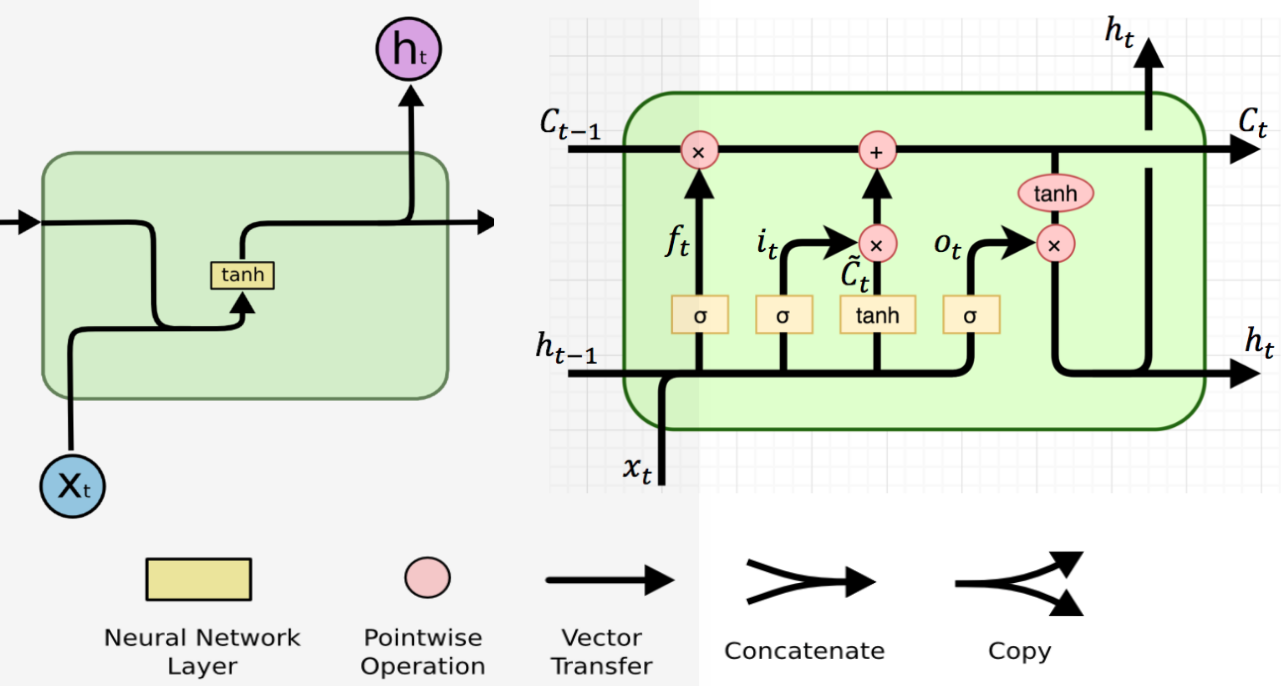
\includegraphics [trim=0 0 0 0, clip, angle=0, width=1.0\columnwidth,
	keepaspectratio]{figures/rnn_lstm}
	\caption{Activation cell of a traditional RNN (top) and a LSTM (bottom)~\cite{colah_lstm}. LSTM propagates the cell $c_t$ and hidden $h_t$ state. With ignoring the forget gate $f_t$, $c_t$ is only updated by sum operations. The gradient along a sum-operation splits up equally and thereby allows to propagate until the beginning of the sequence without vanishing. ResNets have introduced a similar change in the CNN architecture (resnet paper).} 
	\label{fig:rnn_lstm} 
\end{figure}

%TODO take graph of graves paper.
The LSTM is computed according to the following composite function~\cite{DBLP:journals/corr/Graves13}:
\begin{equation}
\begin{aligned}
& i_t = \sigma(W_{xi}x_t + W_{hi}h_{t-1} + W_{ci}c_{t-1} + b_i)\\
& f_t = \sigma(W_{xf}x_t + W_{hf}h_{t-1} + W_{cf}c_{t-1} + b_f)\\
& c_t = f_tc_{t-1} + i_ttanh(W_{xc}x_t + W_{hc}h_{t-1} + b_c)\\
& o_t = \sigma(W_{xo}x_t + W_{ho}h_{t-1} + W_{co}c_{t-1} + b_o)\\
& h_t = o_ttanh(c_t)
\end{aligned}
\label{eq:lstm_eq} 
\end{equation}
where $\sigma$ is the sigmoid function, $i_t$, $f_t$, $o_t$ and $c_t$ are the input gate, forget gate, output gate and cell activation vectors.
The weight matrices are subscripted according to gate names, (e.g. $W_{hf}$ is the hidden-forget weight matrix).
Figuratively speaking, the input gate regulates how much information is taken from the new input $x_t$.
The forget gate can erase the cell memory and thereby controls the duration of time dependency during sequence prediction.
The cell state is the part of memory that propogates between hidden nodes.
The output gate regulates how much information from the hidden cell state is propagated into the output hidden state.

\subsection{LSTMs for binary classification}
We used LSTM networks for the same binary classification task from~\cref{sec:svm}.
LSTMs are able to extract the sequential information more naturally than SVM, so we expected to see better classification accuracy in the train and test datasets.
We used Python and the $\textit{Tensorflow}$ library to implement the LSTMs.

Again, the full trajectories have been precompiled into snippets of static sequence length $T$.
At each time step, the input vector is the relative pedestrian position at time $t$: $x_t \in \Re^{1\text{x}2}$.
For binary classification, we use a many-to-one architecture.
The output is calculated at the output layer by using a logistic sigmoid for binary classification:
\begin{equation}
y_t = \sigma(W_{hout}h_t + b_out)
\label{eq:bin_class_out} 
\end{equation}
where $y_t \in [0,1]$, $W_{hout} \in \Re^{n_{hidden} \text{x} 1}$, and $n_{hidden}$ is the number of hidden units.
The weight matrices and biases are initialized with random noise $\sim\mathcal{N}(0,1)$.
We use the least mean squared error (LMSE) loss function.
The network is optimized by a stochastic gradient descent (SGD) method with the goal to minimize the loss over the weight matrices and their biases.

\subsection{Hyperparameters}
Again, there are many hyperparameters to optimize, including the number of hidden units, batch size, learning rate, and number of training epochs.
It is very time intensive to search over all hyperparamters.
We briefly summarize the hyperparameters' effects on performance, using validation accuracy as the performance metric.
The output of our full grid search is in our posted code (file: rnn\_classifier\_hyperparameters.txt).

The best hyperparameters were batch size of 5, $n_{hidden}=256$, $T=10$, and 3 training epochs, and we used a learning rate of 0.001.

Performance generally levels off after 3-5 training epochs.
For large T, more hidden units are required to handle the higher dimension of the input data.
Specifically, when $T>10$, $n_{hidden}=8$ got $<50\%$ accuracy, but performance improved with $n_{hidden}=64$ (we ranged T from 2-50, and $n_{hidden}$ from 8-256).
Small batch size tended to improve the performance, but it was not a clear trend (we ranged batch size from 1-10).

We also investigate the effect of training set size on performance in~\cref{fig:svm_num_datapts}.
The blue line corresponds to the LSTM classifier, which is not greatly affected by training set size (close to 80\% throughout).
The LSTM classifier is not as sensitive as SVM to training set size. 

\subsection{Results}
After optimizing hyperparameters and confirming we have a sufficient amount of training data, we trained the LSTM binary classifier.
The overall test accuracy was 80.4\%.

The results of the two classifiers (\cref{fig:svm_labels} \& \cref{fig:rnn_labels}) look pretty similar.
The LSTM classifier performed worse than the SVM classifier (84 vs. 80\% test accuracy), which we did not expect.
Both classifiers learned about the ``cross zone'', perform relatively well on data that is predicted to be class 0, and struggle with false negatives far from the vehicle.
The fact that both classifiers performed well/poorly on the same types of data indicates that the data itself was particularly challenging.
Based on our observations of the training data set and classifier performance, it is likely that for many of the snippets that were far from the vehicle, there were similar snippets with each label, which is highly confusing to the classifiers.

\begin{figure}
\centering
\begin{subfigure}{.25\textwidth}
  \centering
  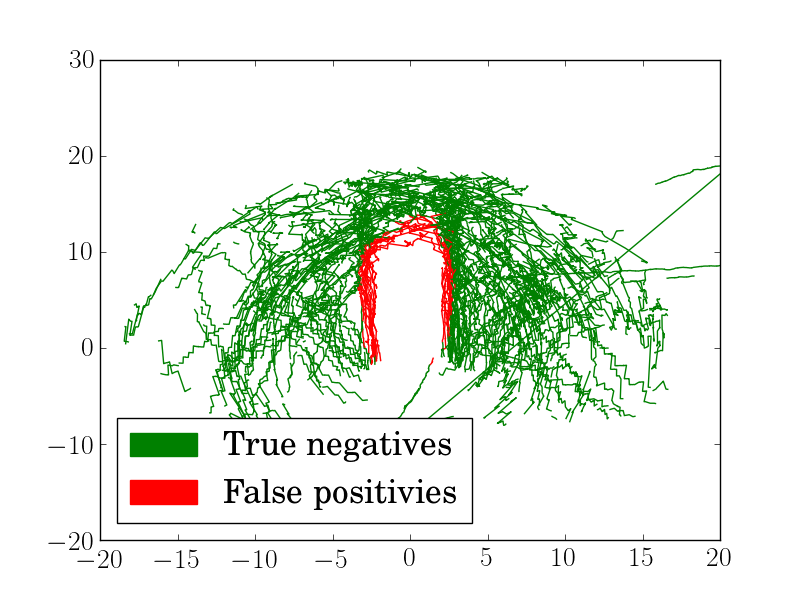
\includegraphics[width=.9\linewidth]{figures/rnn_label0}
  \caption{Trajs. labeled ``No Cross''}
  \label{fig:rnn_label0}
\end{subfigure}%
\begin{subfigure}{.25\textwidth}
  \centering
  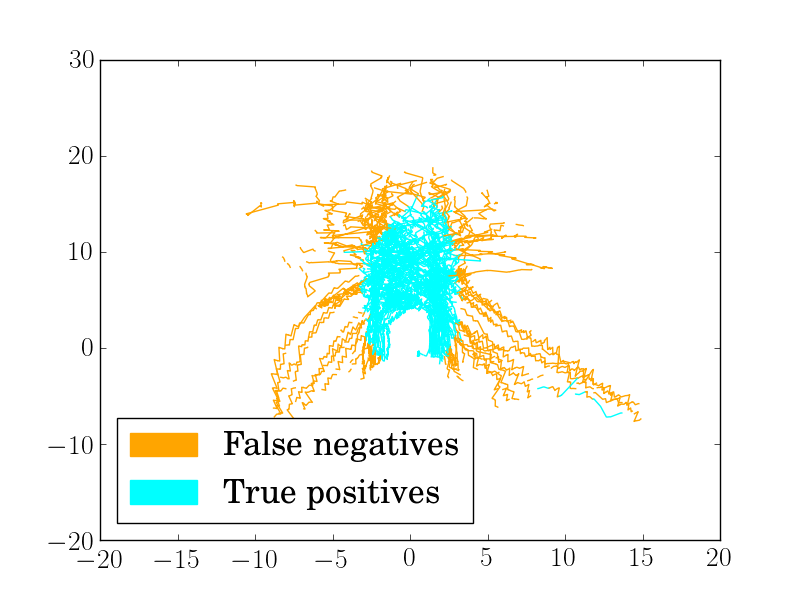
\includegraphics[width=.9\linewidth]{figures/rnn_label1}
  \caption{Trajs. labeled ``Cross''}
  \label{fig:rnn_label1}
\end{subfigure}
\caption{Predicted labels on test set with LSTM classifier. On the left, trajectory snippets that were predicted label 0 (green is correct, red is incorrect). On the right, trajectory snippets that were predicted label 1 (cyan correct, orange incorrect). Across the whole test set, 80\% accuracy was achieved. Compare with~\cref{fig:svm_labels}}
\label{fig:rnn_labels}
\end{figure}

%TODO Figure 4: trajectories are not continuous because of snipping them. That's why a red traj is red and outside the collision area.

\section{Recurrent Neural Network: Prediction} \label{sec:rnn_pred}

\subsection{Introduction}
Previous work has been conducted in predicting trajectories in a 2D space. The most relevant work has used LSTMs to generate human handwriting from the IAM online handwriting database (graves).

LSTMs have the possibility to predict sequences, by feeding themselves their output as an input. To update from binary classification to trajectory predicting LSTM, we change the network architecture from many-to-one to many-to-many. Our output $y_t \Re^{Tx2}$ is computed from every time step as given in ~\cref{eq:eq:bin_class_out}. 

Many work is found on predicting text (hinton,2011). However, our application domain is real-valued in comparison to the discrete valued domain of predicted words.

The literature proposes several transformations, which could be applied instead to the output $y_t$. For example, (Graves) uses mixture density networks (MDNs) and calculates $x_{t+1}$ by the conditional probability $P(x_{t+1}|y_t, )$ and using a Gaussian mixture prior on the probability distribution. The loss is the negative-log likelihood of the conditional probability and SGD is applied to update the weights along with the parameters of the distribution: mean $\mu_m$, standard deviation $\sigma_m$, correlation $\rho_m$, mixture weights $\pi_m$ for $M$ mixture components. However, the complexity of the proposed transition function is obvious and results in longer training time. Due to our limited CPU capacity and corresponding time-consumption of hyperparameter tuning, this approach does not seem promising. 

Additionally, (graves) has used the relative position $\delta x = x_{t+1} - x_t$ as input vector. In our case, we cannot use the relative position, because we would lose the information of proximity to the car. In other words, we would ignore, that a pedestrian might avoid a car, when it approaches him. For the MDN approach our means $\mu_m$ would be further spread among the full absolute position space, which would presumably consume even longer training time with graves approach. Therefore, we have decided to linearly compute the output, as stated in ~\cref{eq:bin_class_out}. 

As we cannot use the loss function proposed by (graves), we have used our loss function, which is the mean squared error over the full output vector and the next ground truth input vector. We have used the $L_2$ norm instead of the $L_1$ norm to be more robust against outliers.

\begin{equation}
Loss_{pred}(x_t) = \frac{1}{T} \sum_{t=0}^{T}(y_t - x_{t+1})^2
\label{eq:loss_pred} 
\end{equation}
%TODO write about last point.

% random batch
The loss function is computed for every batch and updates the parameters in the activation cells via SGD. We randomly draw batches from our training dataset for each SGD parameter update. Thereby we brake apart the dependency of previously concatenated trajectories, that we have split apart into snippets. This is necessary, as a test trajectory will be independent of the training trajectories.

% prediction, parameter-sharing
For prediction, the parameter-sharing property of RNNs and LSTMs is essential. The activation units' parameters have been trained to predict the next state based on the current state. Therefore, for prediction, where the ground truth input vector is unkown, the LSTM can use the output $y_{t-1}$ as input for $x_t$. This gives us the predicted pedestrian position $y_t$.

\subsection{Generated Data}
As seen in the previous sections, the given pedestrian trajectories are highly complex nonlinear functions. To validate our LSTM prediction model, we have trained on the prediction of simpler functions. Therefore, we have chosen to generate linear and sinusodial shaped trajectories, displayed in ~\cref{fig:lin_sin_traj}.

\begin{figure}
	\centering
	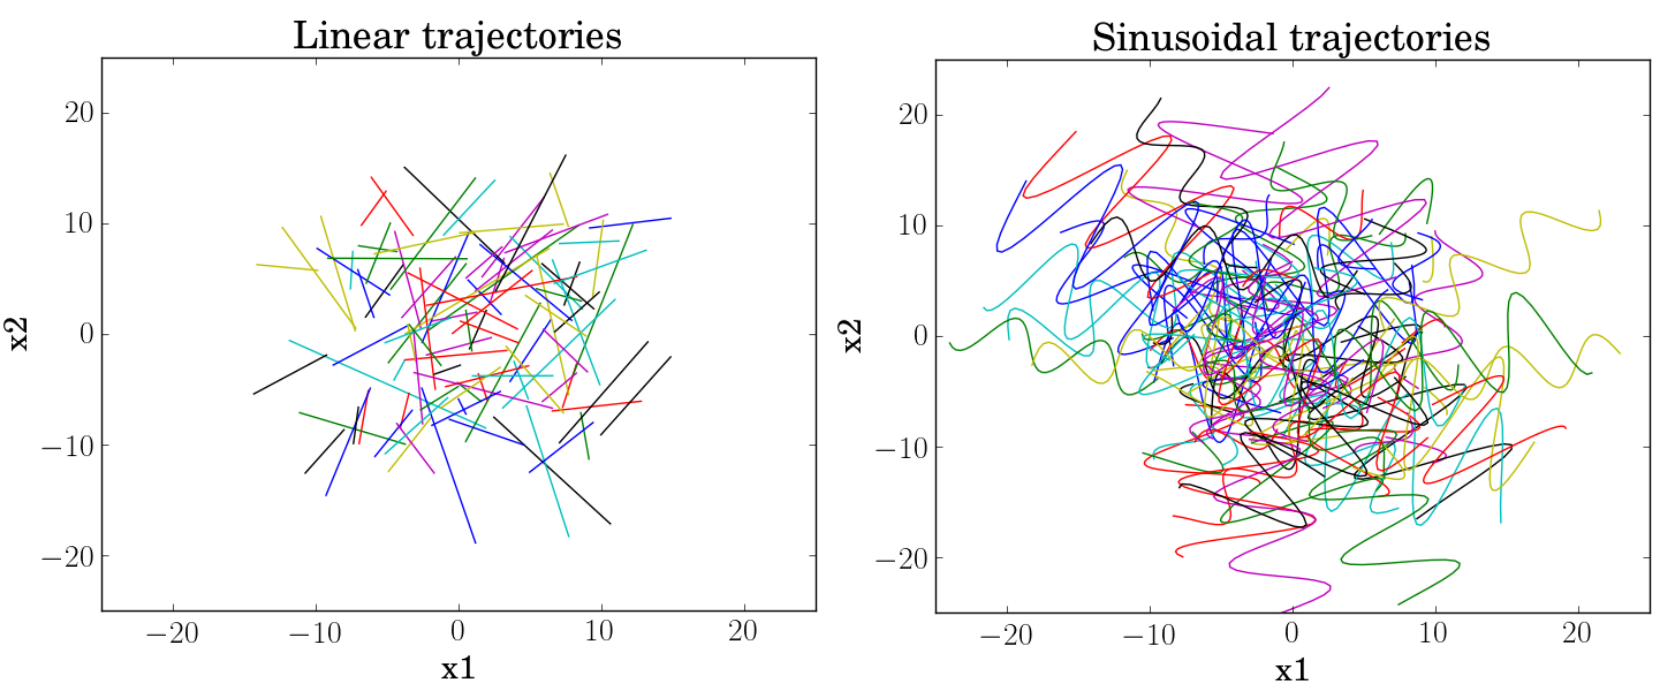
\includegraphics [trim=0 0 0 0, clip, angle=0, width=1.0\columnwidth,
	keepaspectratio]{figures/lin_sin_traj}
	\caption{Randomly generated trajectory data in linear (left) shape and sinusodial shape (right). The trajectories have been generated by sampling the start point, range, scale, translation and rotation at random.} 
	\label{fig:lin_sin_traj} 
\end{figure}
%TODO fit linear data
For our hyperparameter tuning, we have considered the batch size $b$, number of training samples $N$, snippet length $T$, learning rate $lr$, maximum epochs $e_{max}$ and number of hidden units $n_h$. 
As the possible combinations rise exponentially with the number of parameters and our computational resources are very limited, we have evaluated most of the parameters, while holding the other parameters constant. Optimal tuning would run a search over all combinations, which would result in better performance.

Each model is evaluated by the training and validation loss, whereas both datasets are generated independently.

In the search over the number of hidden units we have made the following insights. As seen in ~\cref{fig:rnn_hidden}, the number of hidden units $n_h = 1$ is obviously not sufficient to represent the complexity of sinusodial curves. We can also see, that the complexity of $n_h=4$ is sufficient to fit the sinusodial shape approximately and $n_h=32$ is sufficient to visually exactly fit the data. 

\begin{figure}
	\centering
	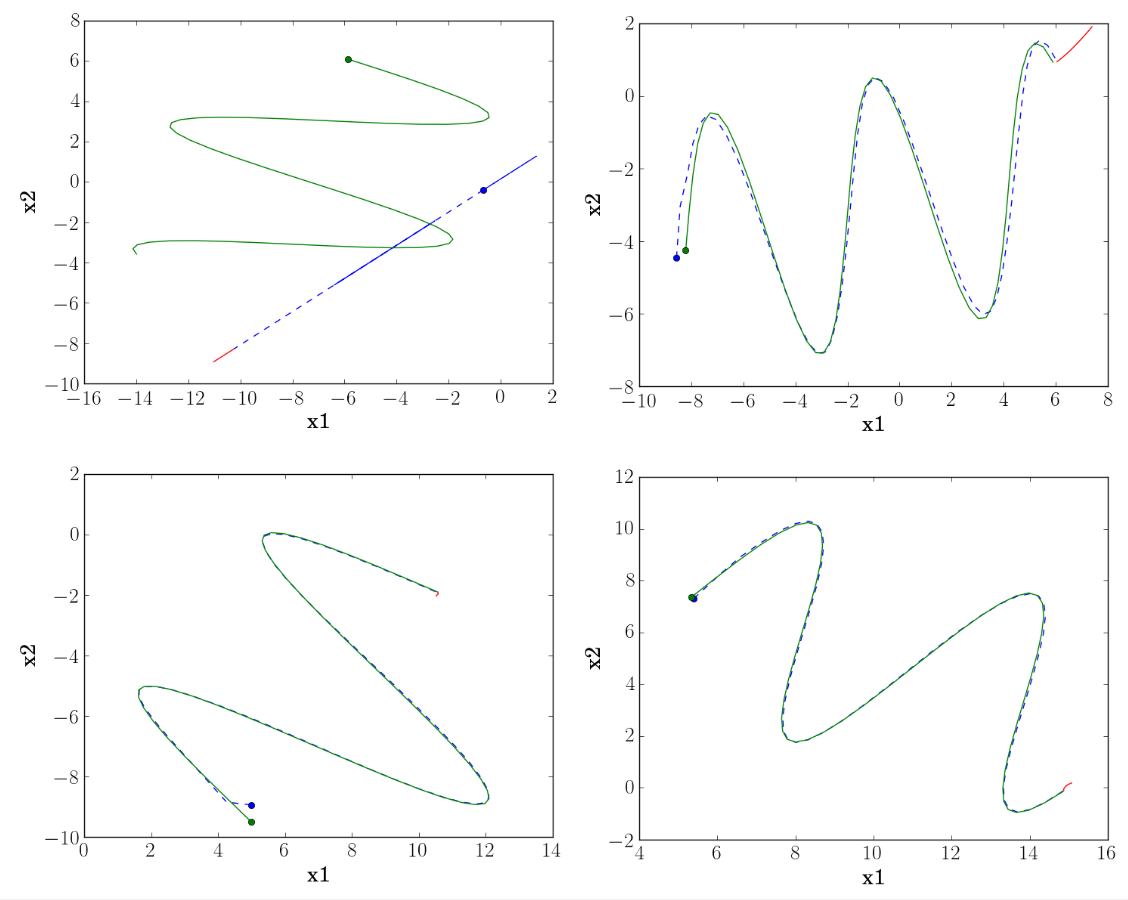
\includegraphics [trim=0 0 0 0, clip, angle=0, width=1.0\columnwidth,
	keepaspectratio]{figures/rnn_hidden}
	\caption{Search over the number of hidden units: $n_h=1$(top-left), $n_h=4$(top-right), $n_h=32$(bottom-left), $n_h=128$(bottom-right). The plot displays the input trajectory (green) $x_t$ with total trajectory snippet length $T=50$ an its starting point (green-dot). The LSTM predicts the next pedestrian position $y_t$ (blue-dotted) with its starting point (blue-dot), based on the past sequence $x_{0:t}$ and the learned parameters. After the input trajectory (green) is finished, the LSTM tries to predict the future trajectory (red) for $T_p=10$ timesteps. All trajectories are test trajectories and have not been included in the training set.}
	\label{fig:rnn_hidden}
\end{figure}

In ~\cref{tab:rnn_hidden} we can see, that increasing the number of hidden nodes $n_h$ shrinks the loss. The training time was exponently increasing with the number of hidden units, which makes us prefer a lower number of hidden units. A high number of hidden units suggests an overfitting on the training data. However, we can see that our independently generated test data shows similar error as the training set. The complexer the model, the less epochs it took to reach acceptable loss. We further refer to the models with the hyperparameters from ~\cref{tab:rnn_hidden} as 1, 4, 32 and 128-unit model.

We have used early stopping, given a validation dataset, to prevent overfitting. The training has been stopped, when the difference in average batch loss between to epochs $\delta L_b < 0.001$.

\begin{table}[]
\centering
\begin{tabular}{ c| c| c| c| c}
& $n_h=1$ & $n_h=4$ &$n_h=32$ & $n_h=128$\\
\hline
$L_e=0$ & 58.5 & 49.7  & \textbf{6.22} & 2.62      \\
$L_e=1$ & 54.2 & 36.0  & \textbf{0.50} & 0.12      \\
$L_e=2$ & 51.1 & 24.4  & \textbf{0.23} & 0.05      \\
$L_e=3$ & 49.2 & 17.8  & \textbf{0.14} & 0.03      \\
\hline
$e_c$ 			& 25 	& 85 	& 35	& 10 		\\
$L_{e_c}$		&  0.30	& 0.03	& 0.0058& 0.004 	\\
$L_{test, e_c}$	& 0.34	& 0.04	&0.003	& 0.003 	\\     
\end{tabular}
\caption{Search over the number of hidden units $n_h$. The average batch loss ($b=100$) over epochs $e$ and test loss is displayed. Number of training samples $N = 5000$ with snippet length $T=50$ and learning rate $lr=0.01$.}
\label{tab:rnn_hidden}
\end{table}

Include oscillating plot for convergence property.
~\cref{fig:rnn_hidden} also illustrates how LSTM starts by guessing $y_0$ purely based on the input $x_0$. 

% minimum snippet length.
Our tuning showed, that the model needs a minimum snippet length to be able to estimate the curve. For very low snippet length ($T<10$) our loss was increasing ($Loss_b=0.02$$ for model $n_h=4$ from ~\cref{tab:rnn_hidden}). An increase in the snippet length over the threshold snippet length $T=50$ was not observed. Therefore, we have set the default snippet length to $T=50$. If we would use RNNs instead of LSTM, the threshold snippet length would be lower, because RNNs have a shorter memory in comparison to LSTMs.

% learning rate, TODO include plot of oscillating learning rate.
The learning rate $lr$ influences the rate of convergence. The higher, the faster the model should converge. However, too high values of the learning rate can cause an oscillation over the minimum. In our case, all learning rates in the interval $[0.1, 0.01, 0.001, 0.0001]$ have been able to find a reasonably low loss. $Lr=0.1$ made the loss oscillate in the interval $[0.01, 0.07]$ for our 32-unit model. A learning rate of $lr=0.01$ for the 32-unit model showed the best tradeoff in terms of minimal loss, while maintaining fast training.

% batch size 
Our choice of batch size $b$ impacted the speed of converges, because tf is possible to execute efficient matrix operations, but did not impact the achievable loss given a fixed model and infinite possible epochs. Given a dataset of the size $N=5000$, we have chosen the batch size to be $b=100$.

%Prediction accuracy.
The LSTM has been designed to predict an unseen pedestrian trajectory for a given number of time steps. Previous work has shown that an LSTM is generally possible to predict a sinusoidial curve into the future (sunsided). However, the found work uses $x_1$ as the input and predicts the $x_2$ value. This is not directly possible in our case, as we have to predict in a local frame with respect to the car. Therefore, we predict both variables at the same time $x = (x_1, x_2)$. Presumably this makes the learning tasks more complex. Additionally, previous work uses more complex models ($n_h=150$) with more training data ($N>500000$) and lower learning rate ($lr<0.0005$). The number of epochs is not stated. An iteration over other hyperparameter choices with these values is not feasible for our computational power and time constraints. Additionally, our domain is more complex. However, the work generally shows that further optimization of the hyperparameters would make it possible to predict trajectories. The red line in ~\cref{fig:rnn_hidden} displays the predictions by our model. 

We conclude that our model is able to predict one step into the future very accurately, given our achieved average batch loss $L_b<0.006$. However, an accurate prediction over many timesteps requires more computational power for hyperparameter tuning. 

\subsection{Real pedestrian data}

We have shown that our LSTM is able continuously predict the next timestep in a domain of translated, rotated, scaled and stretched sinusoidial trajectories. The real pedestrian trajectories are highly nonlinear. LSTMs, in fact neural networks in general, show the capability of fitting a function onto the highly nonlinear data. In ~\cref{fig:ped_data} we can see the trajectories being predicted by our LSTM model.

%TODO add dataset length
We have trained, validated and tested on distinct datasets. All hyperparameters have been chosen based on the results of the sinusodial trajectories and re-validated for the new domain. ~\cref{fig:rnn_real_ped} and ~\cref{tab:rnn_real_ped} shows the performance of our LSTM on real pedestrian data. The learning rate is $lr=0.01$, batch-size $b=100$. 

Additionally, pedestrians behave irrational, do not follow predestined rules and different pedestrians behave differently. 

\begin{figure}
	\centering
	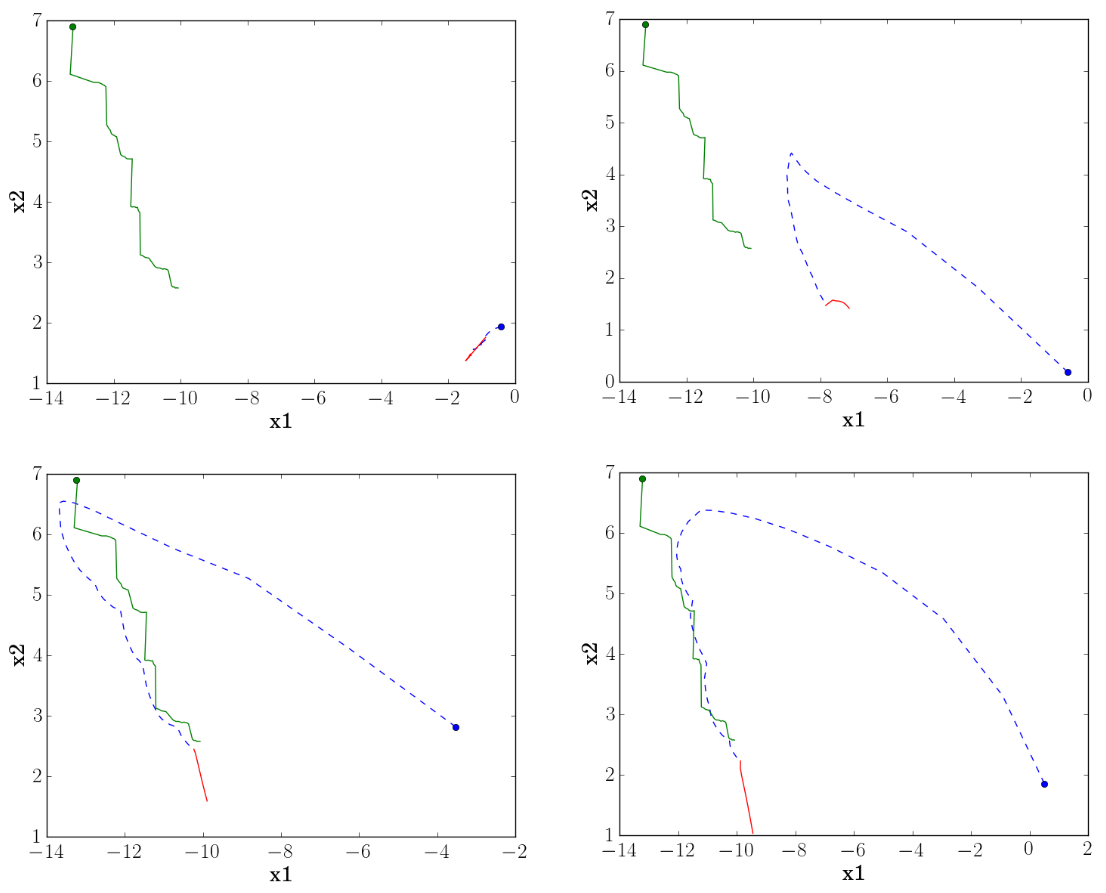
\includegraphics [trim=0 0 0 0, clip, angle=0, width=1.0\columnwidth,
	keepaspectratio]{figures/rnn_real_ped}
	\caption{Search over the number of hidden units: $n_h=1$(top-left), $n_h=4$(top-right), $n_h=32$(bottom-left), $n_h=128$(bottom-right). The plot displays the input trajectory (green) $x_t$ with total trajectory snippet length $T=50$ an its starting point (green-dot). The LSTM predicts the next pedestrian position $y_t$ (blue-dotted) with its starting point (blue-dot), based on the past sequence $x_{0:t}$ and the learned parameters. After the input trajectory (green) is finished, the LSTM tries to predict the future trajectory (red) for $T_p=10$ timesteps. All trajectories are test trajectories and have not been included in the training set.}
	\label{fig:rnn_real_ped}
\end{figure}

\begin{table}[]
\centering
\begin{tabular}{ c| c| c| c| c}
& $n_h=1$ & $n_h=4$ &$n_h=32$ & $n_h=128$\\
\hline
$L_e=0$ & 58.5 & 49.7  & \textbf{6.22} & 2.62      \\
$L_e=1$ & 54.2 & 36.0  & \textbf{0.50} & 0.12      \\
$L_e=2$ & 51.1 & 24.4  & \textbf{0.23} & 0.05      \\
$L_e=3$ & 49.2 & 17.8  & \textbf{0.14} & 0.03      \\
\hline
$e_c$ 			& 25 	& 85 	& 35	& 10 		\\
$L_{e_c}$		&  0.30	& 0.03	& 0.0058& 0.004 	\\
$L_{test, e_c}$	& 0.34	& 0.04	&0.003	& 0.003 	\\     
\end{tabular}


%TODO we have used adam optimizer instead of SGD

\subsection{random stuff}


%TODO oscillating to fit 
In ~\cref{fig:rnn_hidden} (bottom-left), we can see how the error between predicted and true path quickly converges after approximately three timesteps.

The use of dropout is generally not recommended for LSTMs, because it essentially erases parts of the memory. Our tests have shown similar results, where dropout caused results similar to random guessing ~\cref{fig:rnn_dropout}

\begin{figure}
	\centering
	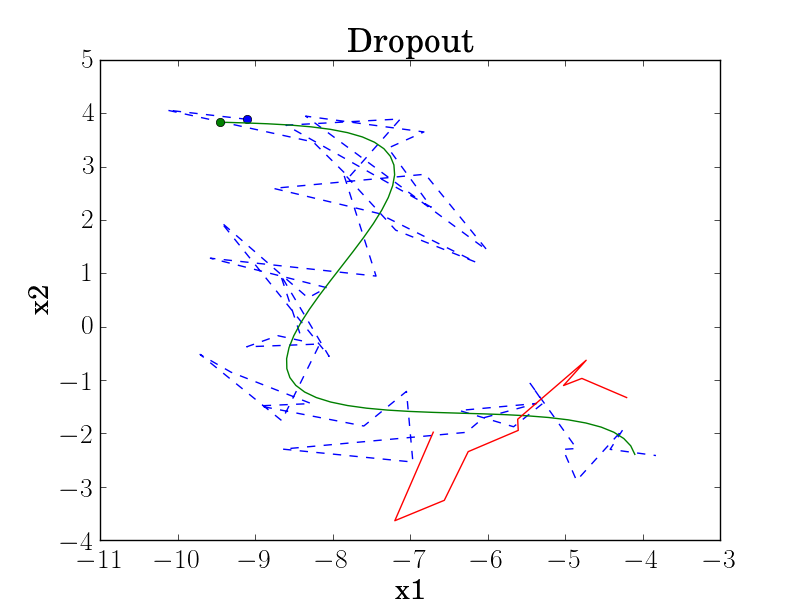
\includegraphics [trim=0 0 0 0, clip, angle=0, width=1.0\columnwidth,
	keepaspectratio]{figures/rnn_dropout}
	\caption{Dropout for LSTMs with dropout rate $d_r = 0.5$. The predicted paths approach random guessing with $mean = x_{t-1}$, $Loss_b = 1.53$ with $b=100$.}
	\label{fig:rnn_dropout}
\end{figure}

\subsubsection{Linear data}

\subsection{Results}



\subsubsection{Hyperparams in bin class}
- Optimize number of hidden units
- batchsize
- learning rate
- maximum epochs


 


- challenge: predict real-valued sequence
- low dimensionality and ease of visualization
- no sophisticated preprocessing or feature-extraction techniques (graves p.18)
	- reduce variation in data (normalize character size, slant, skew,)
- Compare our dataset to handwritten dataset size (graves p.18)
- handwriting has 25 timesteps per character and 700 timesteps per line
- 5000 training, two val of 1500 lines, test 4000 lines (each line 700 tsteps)

\subsection{Network architecture}
- explain $x_t$
	- feeding relative x and y would not respect car position and its influence on pedestrian behavior
- explain $y_t$

\subsection{GRUs}
From: $http://www.jackdermody.net/brightwire/article$
$Sequence_to_Sequence_with_LSTM$

Long Short Term Memory (LSTM) networks are a recurrent neural network that can be used with STS neural networks. They are similar to Gated Recurrent Units (GRU) but have an extra memory state buffer and an extra gate which gives them more parameters and hence a longer training time. While performance with GRU is usually comparable, there are some tasks that each architecture outperforms the other on, so comparing each for a given learning task is usually a good idea.


Number of generated samples: take this from the handwriting paper.
From ~\cref{tab:rnn_hidden}, we have seen how many epochs the model needs to converge. Every epoch repeats training on the same values and thereby increases the probability of overfitting. Therefore, we conclude that we need to train on more data ($N > 5000$), such that the model converges in a low number of epochs and does not overfit.

\subsection{Training}
- Activation unit on output layer
- Optimizer
	- Gradient Descent
		- use momentum?

\subsubsection{Hyperparameters}
- Dropout?!
	- $cell = tf.contrib.rnn.DropoutWrapper(cell, output_keep_prob = args.keep_prob)$

\subsubsection{Regularization}
- Random weight initialization
	- See graves (p.7), weight noise, adaptive weight noise
- use validation set for early stopping
- Gradient clipping?
	- could prove vital for numerical stability
	
\subsection{Results}
- print total loss
- print avg LSE per datapoint


\subsection{Resources}
sunsided $https://github.com/sunsided/tensorflow-lstm-sin$
colah $http://colah.github.io/posts/2015-08-Understanding-LSTMs/$
changhau $https://isaacchanghau.github.io/2017/07/22/LSTM-and-GRU-Formula-Summary/$
hinton 2011 generating text with recurrent neural networks icml 2011
%\listofchanges

%\balance

% \addtolength{\textheight}{-12cm} % This command serves to balance the column lengths
% on the last page of the document manually. It shortens
% the textheight of the last page by a suitable amount.
% This command does not take effect until the next page
% so it should come on the page before the last. Make
% sure that you do not shorten the textheight too much.

%%%%%%%%%%%%%%%%%%%%%%%%%%%%%%%%%%%%%%%%%%%%%%%%%%%%%%%%%%%%%%%%%%%%%%%%%%%%%%%%



%%%%%%%%%%%%%%%%%%%%%%%%%%%%%%%%%%%%%%%%%%%%%%%%%%%%%%%%%%%%%%%%%%%%%%%%%%%%%%%%



%%%%%%%%%%%%%%%%%%%%%%%%%%%%%%%%%%%%%%%%%%%%%%%%%%%%%%%%%%%%%%%%%%%%%%%%%%%%%%%%
\section*{Division of Labor \& Link to code}
Michael mostly worked on the dataset processing and SVM optimization, and Bj{\"o}rn did the RNN work and the rest of the SVM work.
We have been a 2-person team since Milestone 2.
This project is not used for any other classes.
Our code can be found at: \url{https://github.com/mfe7/6.867}.
%%%%%%%%%%%%%%%%%%%%%%%%%%%%%%%%%%%%%%%%%%%%%%%%%%%%%%%%%%%%%%%%%%%%%%%%%%%%%%%%
%\clearpage
\balance
\bibliographystyle{IEEEtran} 
% \bibliographystyle{unsrt} 
\bibliography{biblio}
% \balance
\end{document}
%\grid
